\documentclass[10pt,a4paper,twoside]{report}

\input{../../base/BasePackage.sty}
\input{../../base/OptionsListingC++.sty}

\usepackage{units}
\newcommand{\fig}[1]{Figure.~\ref{#1}}

% Mettre des hyperliens dans le pdf
\hypersetup{pdftitle={Projet Observatoire Pierre Auger},
  pdfsubject={Projet d'informatique - Magistère de Physique Fondamentale},
  pdfauthor={Xavier Garrido, LAL,
    <garrido@lal.in2p3.fr>},
  pdfkeywords={rayons cosmiques, observatoire, Pierre Auger}
}

\begin{document}
\renewcommand{\chaptername}{Projet}

\setcounter{chapter}{3}
\chapter{Détection des rayons cosmiques d'ultra-haute énergie :
  Simulation du détecteur de fluorescence}
\label{projet::opa1}

Les rayons cosmiques forment un fond astrophysique de particules
non-thermiques, supposées chargées, dont les énergies observées
s'étendent du MeV jusqu'à quelques \unit[10$^\text{20}$]{eV}. La détection
dès 1962 d'un rayon cosmique d'énergie supérieure à
\unit[10$^\text{20}$]{eV} par John Linsley et ses collaborateurs sur le
site de Volcano Ranch~\cite{linsley}, a soulevé de
multiples questions qui défient encore la physique contemporaine. Si
l'existence de rayons cosmiques à de telles énergies a été confirmée
par d'autres expériences, ni les nombreux travaux théoriques, ni les
quelques données expérimentales disponibles à ce jour, ne permettent
de comprendre complètement l'origine et la nature de ce rayonnement
hautement énergétique.

La problématique du rayonnement cosmique, en particulier de sa
composante à ultra-haute énergie ($E\geq\unit[10^{18}]{eV}$), se
présente à la fois sous des aspects théoriques,
phé\-no\-mé\-no\-lo\-gi\-ques et observationnels. D'une part, les
astrophysiciens peinent à identifier les sources et les mécanismes
d'accélération capables de porter des protons ou des noyaux du milieu
interstellaire à des énergies aussi extrêmes. D'autre part,
l'interaction de ces astroparticules avec le fond diffus cosmologique,
qui intervient lors de leur propagation dans l'Univers, devrait
entraîner la suppression de leur flux au delà de
$\unit[10^{20}]{eV}$. Cette caractéristique du spectre en énergie
connue sous le nom de coupure GZK~\cite{greisen, zatsepin}, est
étroitement liée à toute la physique spéculative qui gravite autour de
l'existence même de ces rayons cosmiques d'ultra-haute
énergie~(RCUHE). Enfin, la rigidité de ces particules, à savoir le
rapport de leur énergie sur leur charge, conjuguée à la supposée
faible intensité du champ magnétique extragalactique et à la
connaissance raisonnable de sa composante galactique, rendent
pertinentes les tentatives de corrélation entre leurs directions
d'arrivées et leurs sites de production.

La principale limitation technique tient à la rareté des RCUHEs
$-$~typiquement 1 particule par km$^2$ et par siècle à
$\unit[10^{20}]{eV}$~$-$ impliquant la mise en \oe uvre d'une surface
de détection exceptionnelle pour recueillir un nombre d'événements
statistiquement représentatif. Par ailleurs, l'observation des rayons
cosmiques se fait au travers de l'étude des cascades de particules
secondaires, conséquence du passage de ces corpuscules extrêmes au
sein de l'atmosphère : les propriétes du rayonnement cosmique sont
donc indirectement déduites de l'étude des gerbes
atmosphériques. Grâce à la combinaison d'un réseau de 1600 cuves à
effet Cherenkov associé à 24 télescopes de fluorescence,
l'Observatoire Pierre Auger peut observer simultanément le
dévelop\-pement longitudinal et latéral des gerbes atmosphériques. Le
couplage de ces deux techniques permet d'affiner les reconstructions
géométriques, d'intercalibrer les détecteurs et d'évaluer, en
conséquence, les éventuels biais inhérents à chaque mode de
détection. En outre, la surface couverte par le détecteur de surface
voisine de $\unit[3000]{km^2}$ fait de cet instrument le plus grand
détecteur de rayons cosmiques jamais construit.

\begin{figure}
  \centering
  \begin{tabular}{cc}
    \multicolumn{2}{c}{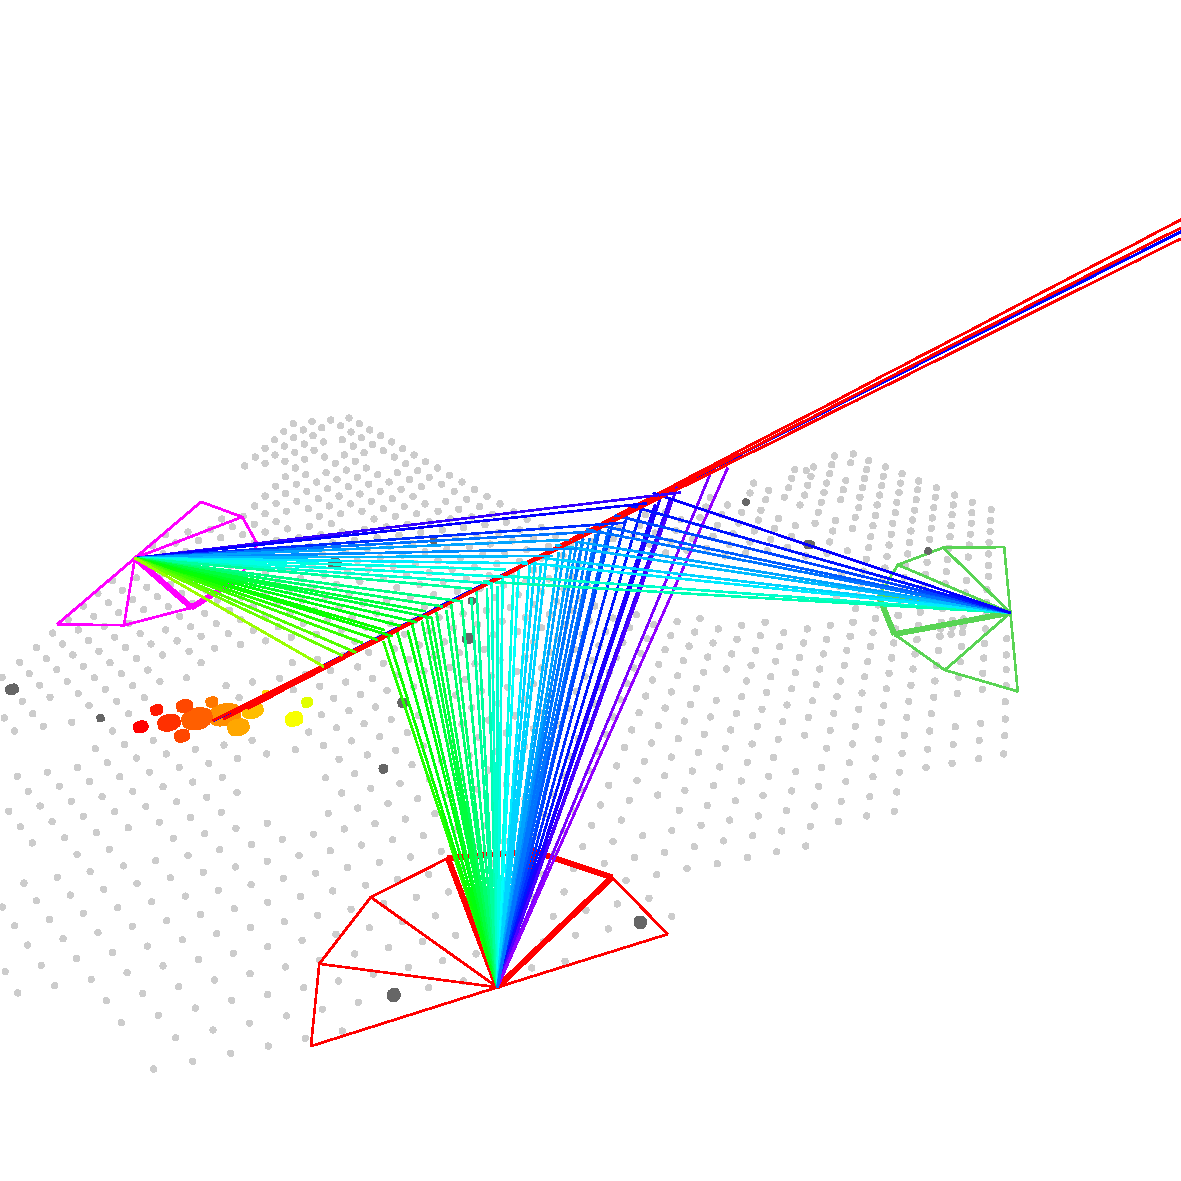
\includegraphics[scale=0.4]{./plot/AugerEvent_200812301774}}\\
    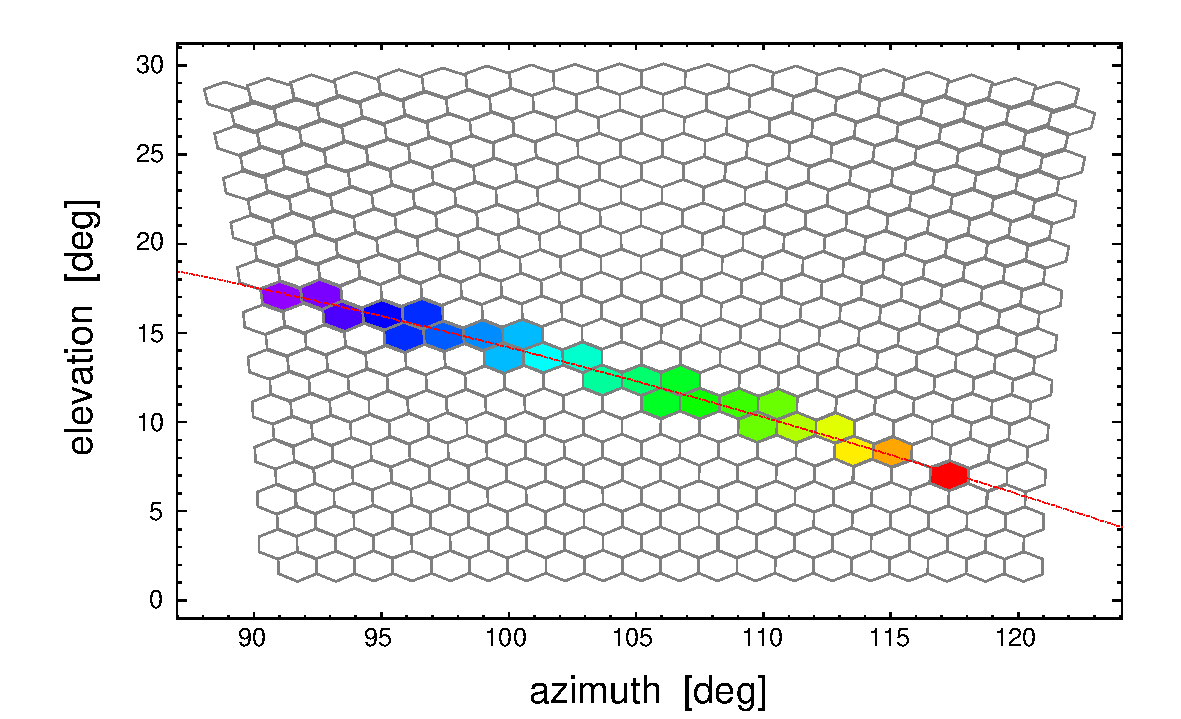
\includegraphics[scale=0.35]{./plot/camera} &
    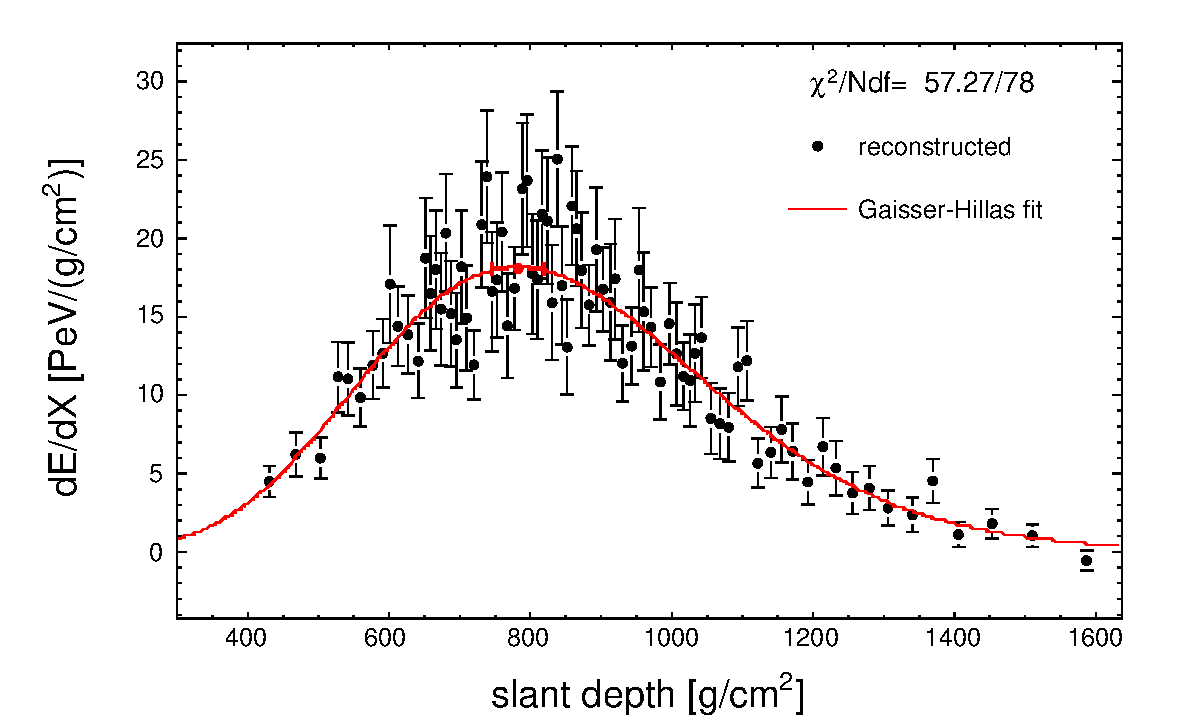
\includegraphics[scale=0.35]{./plot/gh}
  \end{tabular}
  \caption{\textbf{\label{fig::rec}Vue 3D d'un événement hybride observé par
      l'Observatoire Pierre Auger~(figure du haut). Réponse d'une
      caméra d'un détecteur de fluorescence~(figure de gauche) et
      profil longitudinal de la gerbe atmosphérique~(figure de droite).}}
\end{figure}

\section{Présentation du projet}

Le but de ce projet est de simuler la réponse du détecteur de
fluorescence lors du passage d'une gerbe atmosphérique. Le rayonnement
de fluorescence est consécutif à l'interaction entre les particules
chargées de la gerbe $e^-/e^+$ et l'azote présent dans
l'atmosphère : le rayonnement UV (\unit[300-400]{nm}) résulte de la
désexcitation des atomes d'azote.

Chaque détecteur de fluorescence est composé de 6 caméras comprenant
20$\times$22 pixels~(\emph{cf.}~\fig{fig::rec}). \`A chaque pixel
correspond :

\begin{enumerate}

\item[\textbullet] deux angles ($\theta_i, \phi_i$) où $\theta_i$
  correspond à l'élévation du pixel $(i,j)$ et où $\phi_i$ est l'angle
  azimuthal,
\item[\textbullet] un signal dont la valeur sera vrai ou fausse selon
  que le pixel ait été touché ou non,
\item[\textbullet] un temps $t_{i,j}$ d'arrivée du signal dans le pixel
  $(i,j)$.

\end{enumerate}

La caméra couvre un champ de 30\textdegree~par 33\textdegree. Le
pixel ($i,j$) pointe ainsi dans la direction :
\begin{equation*}
\theta_i=1.5\times j \quad \text{et} \quad \phi_j=60 + 1.5\times(20-i)
\end{equation*}
où $i\in[1,20]$ et $j\in[1,22]$.

\subsection{Génération et simulation d'événement}

Un événement est caractérisé par l'énergie~$E$ de la particule
primaire et sa direction ($\theta_\text{SDP}$, $\phi_\text{SDP}$). Le
plan de détection de la gerbe correspond au plan contenant l'axe de la
gerbe et passant par le détecteur de
fluorescence~(\emph{cf.}~\fig{fig::fd}). La distance entre le
détecteur et l'axe de la gerbe est alors notée~$R_p$ tandis
que~$\chi_0$ est l'angle entre le sol et la direction de la gerbe. La
génération des événements consiste à tirer aléatoirement des valeurs
pour les variables précédentes : $R_p$ sera compris entre 8 et
\unit[12]{km}, $\theta_\text{SDP}$ sera tiré uniformément entre 90 et
100 degrés et $\phi_\text{SDP}$ entre 60 et 90 degrés. L'angle
$\chi_0$ variera entre 80 et 100 degrés.

\begin{figure}
  \centering
  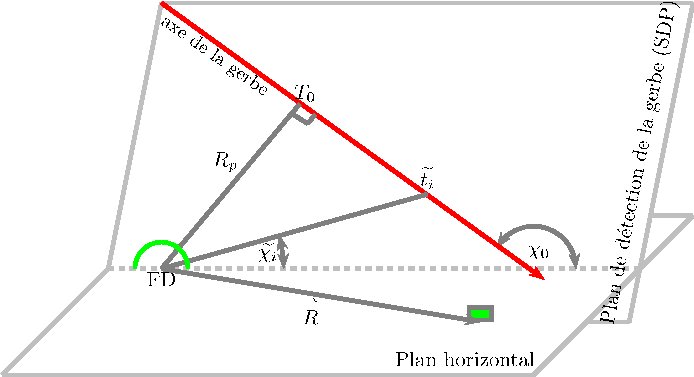
\includegraphics[scale=1.]{./plot/HybridPlan}
  \caption{\textbf{\label{fig::fd}Paramètres géométriques de la gerbe
      pour la reconstruction hybride.}}
\end{figure}

\'Etant donné les paramètres simulés, il s'agit de simuler la réponse
d'une caméra au passage de cette gerbe. L'ensemble des pixels touchés
vérifie l'équation suivante :
\begin{equation}
  \theta_i=\frac{\phi_j-\phi_\text{SDP}}{\tan\,\theta_\text{SDP}}
  \label{eq::theta}
\end{equation}
et le temps d'arrivée est donné par :
\begin{equation}
  t_{(i,j)} = -\frac{R_p}{c}\times\left(\tan(\pi/2 - \chi_0)-\tan(\pi-\chi_0-\theta_i)\right)
  \label{eq::time}
\end{equation}

\subsection{Reconstruction des événements}

\`A partir des informations issues de la caméra, on reconstruira les
valeurs $R_p$, $\theta_\text{SDP}$, $\phi_\text{SDP}$ et $\chi_0$. Les
valeurs de $\theta_\text{SDP}$ et $\phi_\text{SDP}$ se déduisent de
l'équation~\ref{eq::theta} en ajustant les données $(\theta_i,
\phi_j)$. De même, les paramètres $R_p$ et $\chi_0$ sont obtenus à
partir du temps de chacun des pixels $(i,j)$. On comparera ces données
reconstruites aux valeurs simulées.

Dans un second temps, on pourra simuler le bruit de la caméra à savoir
le fait que certains pixels déclenchent sans rapport avec le passage
d'une gerbe atmosphérique. La position de ces pixels est aléatoire et
le temps sera compris dans une fénêtre de \unit[5]{$\mu$s} entre le
premier et le dernier pixel touché. On ajoutera donc ce bruit de pixel
(entre 1 et 10 pixels bruyants) et on évaluera l'impact sur la qualité
de la reconstruction. On pourra enfin envisager de supprimer ce bruit
en fonction de critères de cohérence spatiale et/ou temporelle.

\def\etal{\textit{et al.}}

\renewcommand{\bibname}{References}

\begin{thebibliography}{9}
  \bibliographystyle{unsrt}

\bibitem{linsley} J.~Linsley, {\em Evidence for a Primary Cosmic-Ray
  Particle with Energy 10$^{20}$ eV}", Physical Review Letters,
  vol. 10, pp 146-148 (1963)

\bibitem{greisen} K.~Greisen, {\em End to the Cosmic-Ray Spectrum ?},
  Physical Review Letters, vol. 16, pp 748-750 (1966)

\bibitem{zatsepin} G.~T.~Zatsepin and V.~A.~Kuz'min, {\em Upper Limit
  of the Spectrum of Cosmic Rays}, Soviet Journal of Experimental and
  Theoretical Physics Letters, vol. 4, pp 78 (1966)

\end{thebibliography}


\end{document}

% Local Variables:
% mode: latex
% coding: utf-8-unix
% End:
